\section{Parallel collision handling}
\label{sec:parallel-contact}
We prevent collisions of \rbcs with other \rbcs and with the vessel
surface $\Gamma$ by solving the \ncp given in \cref{eq:ncp1,eq:ncp2}. 
This is a nonsmooth and non-local problem, whose assembly and efficient solution
is particularly challenging in parallel.%, especially in the context of complex geometries. 
In this section, we summarize our constraint-based approach and algorithm.

We have integrated piecewise polynomial patches into the framework of \cite{lu2018parallel} 
for parallel collision handling, to which we refer the reader for a more detailed discussion. 
The key step to algorithmically unify \rbcs and patches is to \textit{form a linear triangle
mesh approximation} of both objects.
We now want to enforce that these meshes are collision-free subject to the
physics constraints in \cref{eq:ncp1}.

%Rather than try to solve the original \ncp problem directly,
We linearize the \ncp
and solve a sequence of \lcps whose solutions converge
to the \ncp solution.
At a high-level, the collision algorithm proceeds as follows:
\begin{enumerate}
    \item\label{step:near_tri_pair} Find triangle-vertex pairs of distinct meshes that are candidates for collision.
    \item Compute $V(t^+) = V(t^{+,0})$. If any triangle-vertex pairs on distinct meshes collide, the corresponding component of $V(t)$ will be negative.
    \item While $V_i(t^{+,k}) < 0$ for any $i$:
    \begin{enumerate}
        \item Suppose $m$ components of $V(t)$ are negative 
        \item \label{step:lcp_solve} Solve the following linearized version of \cref{eq:ncp1,eq:ncp2}
    \begin{align}
      \vX^{+,k}_i &= \vX_i + \Delta t (\vb_i + S_i(\vfd_i(\vX_i^{+,k},\lambda^{+,k})),\label{eq:ncp1}\\
      \lambda(t^+) \geq 0, &\quad  L(t^{+,k})\geq 0,
      \quad \lambda(t^{+,k}) \cdot L(t^{+,k}) 
      = 0,\label{eq:ncp2}\\
      &\text{where}\quad L(t) = V(t) + \nabla_u V^T \Delta \vX_i(t)
    \end{align}%
    for the $k$th iteration of the loop and $\vX^{+,k}_i = \vX_i +
    \Delta\vX_i(t^{+,k})$. 
  \item Find new candidate triangle-vertex pairs and compute $V(t^{+,k})$.
    \end{enumerate} 
\end{enumerate}
Here, $t^{+,k}$ is the intermediate time step at which a new candidate position $\vX_i^{+,k}$ occurs.
This approach of iteratively solving an \ncp with sequence of \lcps was shown to converge superlinearly in \cite{fang1984linearization}. 
%Our integration time stepping is small enough to appromixate STV V with linearizations.
In \cite{yan2019computing}, the authors demonstrate that one \lcp linearization can approximate the \ncp accurately; our algorithm uses around seven \lcp solves to approximately solve the \ncp.
Upon convergence of this algorithm, we are guaranteed that our system is collision-free.

\begin{figure}[h]
\centering
\begin{minipage}[b]{0.8\textwidth}
    \centering
    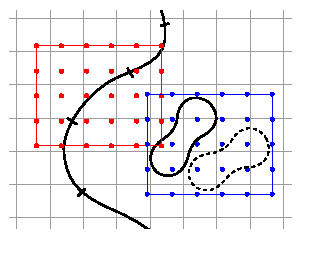
\includegraphics[angle=0,width=.7\linewidth]{figs/grid_and_check_points.pdf}
  \mcaption{fig:grid-search}{A \twod depiction of the parallel candidate collision
    pair algorithm}{ Shown is the implicit spatial grid (gray), a piece of the
blood vessel $\Gamma$ (open black curve), an \rbc $\gamma_i$ at the current time
step (closed black curve) and at the next time step (dotted closed back curve).
Also shown is the space-time bounding box and bounding box samples of a single
patch (red square and red dots) and an \rbc (blue square and blue dots).
}
\end{minipage}
\end{figure}%
To solve the \lcp in \cref{step:lcp_solve}, we follow the approach
detailed in \cite[Section 3.2.2, Section 3.3]{lu2017}. 
We reformulate the problem first in standard \lcp form with diagonally-dominant system matrix $\vB$, then 
solve an equivalent root finding problem by applying a minimum-map Newton's
method. This can be restructured to use \gmres, so we only need to repeatedly apply  
$\vB$ to vectors to solve the \lcp.
Each entry $\vB_{ij}$ is the change in the $j$th contact volume induced by the
$k$th contact force, which is explicitly defined in
\cite[Algorithm 3]{lu2018parallel}.
This means that $\vB$ is of size $m \times m$, where $m$ is the number of
collisions, but is extremely sparse.
We need not store the entire matrix explicitly; we only compute the non-zero entries and
store them in a distributed hash-map.
Computing these matrix elements requires an accumulation of all coupled
collision contributions to the velocity, which requires just a sparse
\texttt{MPI\_All\_to\_Allv} to send each local contribution to the process containing
$V_i(t^{+,k})$.

An important step to ensure good scaling of our collision handling algorithm is
to minimize the number of triangle-vertex pairs that are found in
\cref{step:near_tri_pair}. One could explicitly compute an
all-to-all collision detection on all meshes in the system, but this requires
$O(N^2)$ work and global communication.
We perform a high-level filtering first to find local \textit{candidate collision
mesh pairs}, then only communicate and compute the required $O(m)$ information.
Since spatially-near mesh pairs may be on different 
processors, we need a parallel algorithm to compute these collision candidates.

To address this, we reuse \cref{step:bbnear,step:computeid,step:sort} from
\cref{sec:closest_point} and adapt it to this problem. For each mesh in the
system, we form the \textit{space-time
  bounding box} of the mesh: the smallest axis-aligned bounding box
containing the mesh at positions $\vX_i$ and $\vX_i^+$, as shown in
\cref{fig:grid-search}.  For patches $P_i$, note that $P_i^+ = P_i$.
This means one can reuse the bounding box of $P_i$ constructed in
\cref{sec:closest_point} for this purpose and simply set $d_\eps$ to zero.
After forming all space-time bounding boxes for the meshes of all patches and \rbcs, we
apply steps \cref{step:computeid,step:sort} directly to these boxes.
\cref{step:sort} will communicate meshes with the same spatial sorting key to
the same processor; these meshes are collision candidate pairs.
Once the computation is local and candidate collision pairs are identified, we
can proceed with the
\ncp solution algorithm described above.


